
\subsection{Random intercept variance}
\begin{figure}[H]
  \centering
  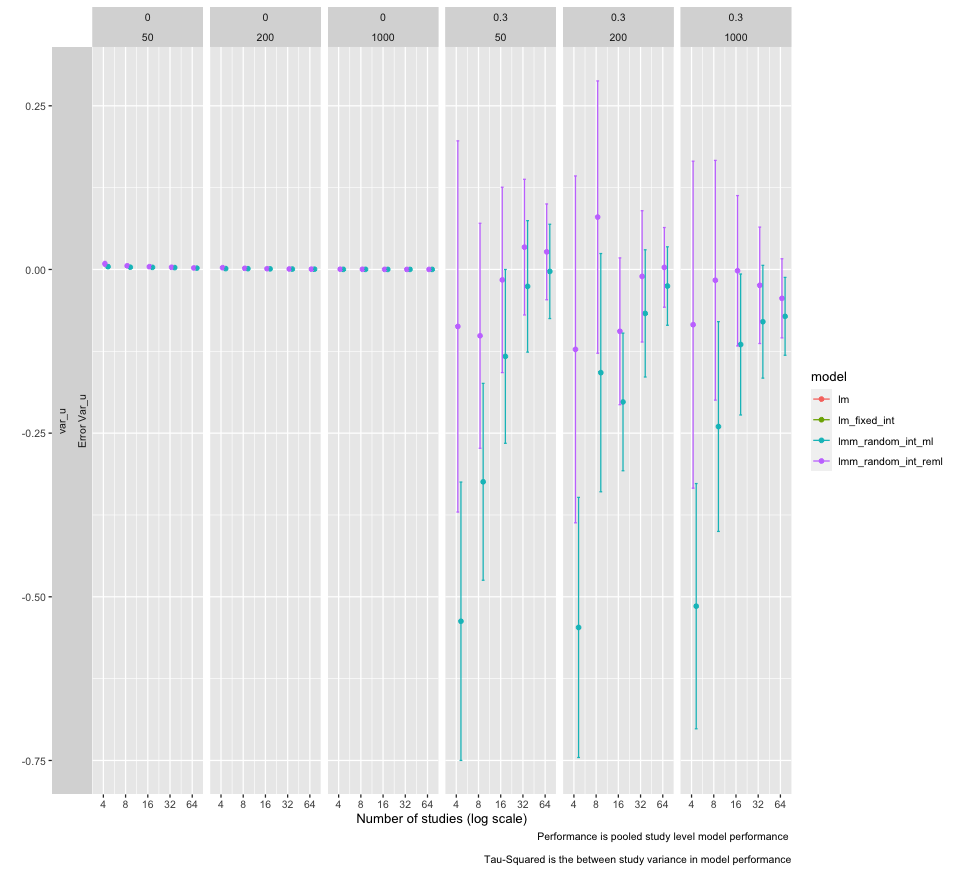
\includegraphics[width=1\linewidth]{Ch05: Simulations/supp_plots/supp_mat_pt1/var_u.pdf}
  \caption{Estimated random intercept variance}
\end{figure}

\subsection{Pooled calibration in the large}
\begin{figure}[H]
  \centering
  \includegraphics[width=1\linewidth]{Ch05: Simulations/supp_plots/supp_mat_pt1/calib_itl4.pdf}
  \caption{Calibration in the large, training data 4 studies}
\end{figure}

\begin{figure}[H]
  \centering
  \includegraphics[width=1\linewidth]{Ch05: Simulations/supp_plots/supp_mat_pt1/calib_itl8.pdf}
  \caption{Calibration in the large, training data 8 studies}
\end{figure}

\begin{figure}[H]
  \centering
  \includegraphics[width=1\linewidth]{Ch05: Simulations/supp_plots/supp_mat_pt1/calib_itl16.pdf}
  \caption{Calibration in the large, training data 16 studies}
\end{figure}

\begin{figure}[H]
  \centering
  \includegraphics[width=1\linewidth]{Ch05: Simulations/supp_plots/supp_mat_pt1/calib_itl32.pdf}
  \caption{Calibration in the large, training data 32 studies}
\end{figure}

\subsection{Between-study hetrogeneity in calibration in the large}
\begin{figure}[H]
  \centering
  \includegraphics[width=1\linewidth]{Ch05: Simulations/supp_plots/supp_mat_pt1/calib_itl_hetro4.pdf}
  \caption{Hetrogeneity in Calibration in the large, training data 4 studies}
\end{figure}

\begin{figure}[H]
  \centering
  \includegraphics[width=1\linewidth]{Ch05: Simulations/supp_plots/supp_mat_pt1/calib_itl_hetro8.pdf}
  \caption{Hetrogeneity in Calibration in the large, training data 8 studies}
\end{figure}

\begin{figure}[H]
  \centering
  \includegraphics[width=1\linewidth]{Ch05: Simulations/supp_plots/supp_mat_pt1/calib_itl_hetro16.pdf}
  \caption{Hetrogeneity in Calibration in the large, training data 16 studies}
\end{figure}

\begin{figure}[H]
  \centering
  \includegraphics[width=1\linewidth]{Ch05: Simulations/supp_plots/supp_mat_pt1/calib_itl_hetro32.pdf}
  \caption{Hetrogeneity in Calibration in the large, training data 32 studies}
\end{figure}

\subsection{Pooled calibration slope}
\begin{figure}[H]
  \centering
  \includegraphics[width=1\linewidth]{Ch05: Simulations/supp_plots/supp_mat_pt1/calib_slope4.pdf}
  \caption{Calibraiton slope, training data 4 studies}
\end{figure}

\begin{figure}[H]
  \centering
  \includegraphics[width=1\linewidth]{Ch05: Simulations/supp_plots/supp_mat_pt1/calib_slope8.pdf}
  \caption{Calibraiton slope, training data 8 studies}
\end{figure}

\begin{figure}[H]
  \centering
  \includegraphics[width=1\linewidth]{Ch05: Simulations/supp_plots/supp_mat_pt1/calib_slope16.pdf}
  \caption{Calibraiton slope, training data 16 studies}
\end{figure}

\begin{figure}[H]
  \centering
  \includegraphics[width=1\linewidth]{Ch05: Simulations/supp_plots/supp_mat_pt1/calib_slope32.pdf}
  \caption{Calibraiton slope, training data 32 studies}
\end{figure}

\subsection{Between-study hetrogeneity in calibration slope}
\begin{figure}[H]
  \centering
  \includegraphics[width=1\linewidth]{Ch05: Simulations/supp_plots/supp_mat_pt1/calib_slope_hetro4.pdf}
  \caption{Between-study hetrogeneity in calibraiton slope, training data 4 studies}
\end{figure}

\begin{figure}[H]
  \centering
  \includegraphics[width=1\linewidth]{Ch05: Simulations/supp_plots/supp_mat_pt1/calib_slope_hetro8.pdf}
  \caption{Between-study hetrogeneity in calibraiton slope, training data 8 studies}
\end{figure}

\begin{figure}[H]
  \centering
  \includegraphics[width=1\linewidth]{Ch05: Simulations/supp_plots/supp_mat_pt1/calib_slope_hetro16.pdf}
  \caption{Between-study hetrogeneity in calibraiton slope, training data 16 studies}
\end{figure}

\begin{figure}[H]
  \centering
  \includegraphics[width=1\linewidth]{Ch05: Simulations/supp_plots/supp_mat_pt1/calib_slope_hetro32.pdf}
  \caption{Between-study hetrogeneity in calibraiton slope, training data 32 studies}
\end{figure}

\subsection{Pooled R-sqaured}
\begin{figure}[H]
  \centering
  \includegraphics[width=1\linewidth]{Ch05: Simulations/supp_plots/supp_mat_pt1/r2_4.pdf}
  \caption{R-squared, training data 4 studies}
\end{figure}

\begin{figure}[H]
  \centering
  \includegraphics[width=1\linewidth]{Ch05: Simulations/supp_plots/supp_mat_pt1/r2_8.pdf}
  \caption{R-squared, training data 8 studies}
\end{figure}

\begin{figure}[H]
  \centering
  \includegraphics[width=1\linewidth]{Ch05: Simulations/supp_plots/supp_mat_pt1/r2_16.pdf}
  \caption{R-squared, training data 16 studies}
\end{figure}

\begin{figure}[H]
  \centering
  \includegraphics[width=1\linewidth]{Ch05: Simulations/supp_plots/supp_mat_pt1/r2_32.pdf}
  \caption{R-squared, training data 32 studies}
\end{figure}

\subsection{Between-study hetrogeneity in R-squared}
\begin{figure}[H]
  \centering
  \includegraphics[width=1\linewidth]{Ch05: Simulations/supp_plots/supp_mat_pt1/r2_hetro4.pdf}
  \caption{Between-study hetrogeneity in R-Squared, training data 4 studies}
\end{figure}

\begin{figure}[H]
  \centering
  \includegraphics[width=1\linewidth]{Ch05: Simulations/supp_plots/supp_mat_pt1/r2_hetro8.pdf}
  \caption{Between-study hetrogeneity in R-Squared, training data 8 studies}
\end{figure}

\begin{figure}[H]
  \centering
  \includegraphics[width=1\linewidth]{Ch05: Simulations/supp_plots/supp_mat_pt1/r2_hetro16.pdf}
  \caption{Between-study hetrogeneity in R-Squared, training data 16 studies}
\end{figure}

\begin{figure}[H]
  \centering
  \includegraphics[width=1\linewidth]{Ch05: Simulations/supp_plots/supp_mat_pt1/r2_hetro32.pdf}
  \caption{Between-study hetrogeneity in R-Squared, training data 32 studies}
\end{figure}

